\chapter[2021 June]{June 2021}

\section[2021/06/11]{Friday, 11 June 2021}

\subsection{Centroid Detection for Multiple Cubes}

Previous results have shown that segmentation of the top face of the cube based on light intensity offers the most promising avenue to robustly detect and localise the cube. In order to develop this concept further, several adjustments were made to the previous image processing test setups. Firstly, it was previously demonstrated that the introduction of colour information into the image through the addition of a coloured background offers no better performance than pure light intensity information. Therefore, in order to maximise the light intensity differential between the reflective top face of the cube, a plain matte black paper background was introduced. Secondly, it was observed that when the angle between the light incident on the top face of the cube and the light reflected into the camera is minimised, the light intensity on the top face of the cube as observed by the camera is maximised. To make the most of this effect, the camera was placed parallel to the base plane at a height of approximately 500 mm with two bright \ac{LED} lights on either side angled toward the centre of the base plane. Lastly, to test that the ability of the image processing algorithm to detect multiple cubes in the same image with variying top face light intensities, multiple cubes were placed randomly on the base plane.

\FigRef{fig:multiple-cubes} shows the image that was captured with the above setup. Note the light intensity on the top face of each cube. The first step in extracting the contours from the image is to apply binary thresholding to the image to segment the top faces of the cubes. In preparation for this, the image was first converted to grayscale and blurred. The binary threshold in which only pixels with intensities greater than 140 out of 255 were retained. This resulted in a well segmented collection of cube top faces. The OpenCV contour detection algorithm was then applied to this binary images which resulted in the red contours shown in \FigRef{fig:multiple-cube-centroids}. Finally, the moment of each contour was calculated and used to find the centroid of each face. These centroids are indicated as blue dots in \FigRef{fig:multiple-cube-centroids}. All the cube centroids were successfully detected in terms of the image coordinate system which is sufficient output from the object detection phase. Methods to attain the vertices of the upper face will still be explored with the intent of use in pose estimation. The next process to be investigated needs to be capable of mapping these image coordinates to the world coordinate system.

\begin{figure}[H]
    \centering
    \begin{subfigure}[b]{0.45\textwidth}
         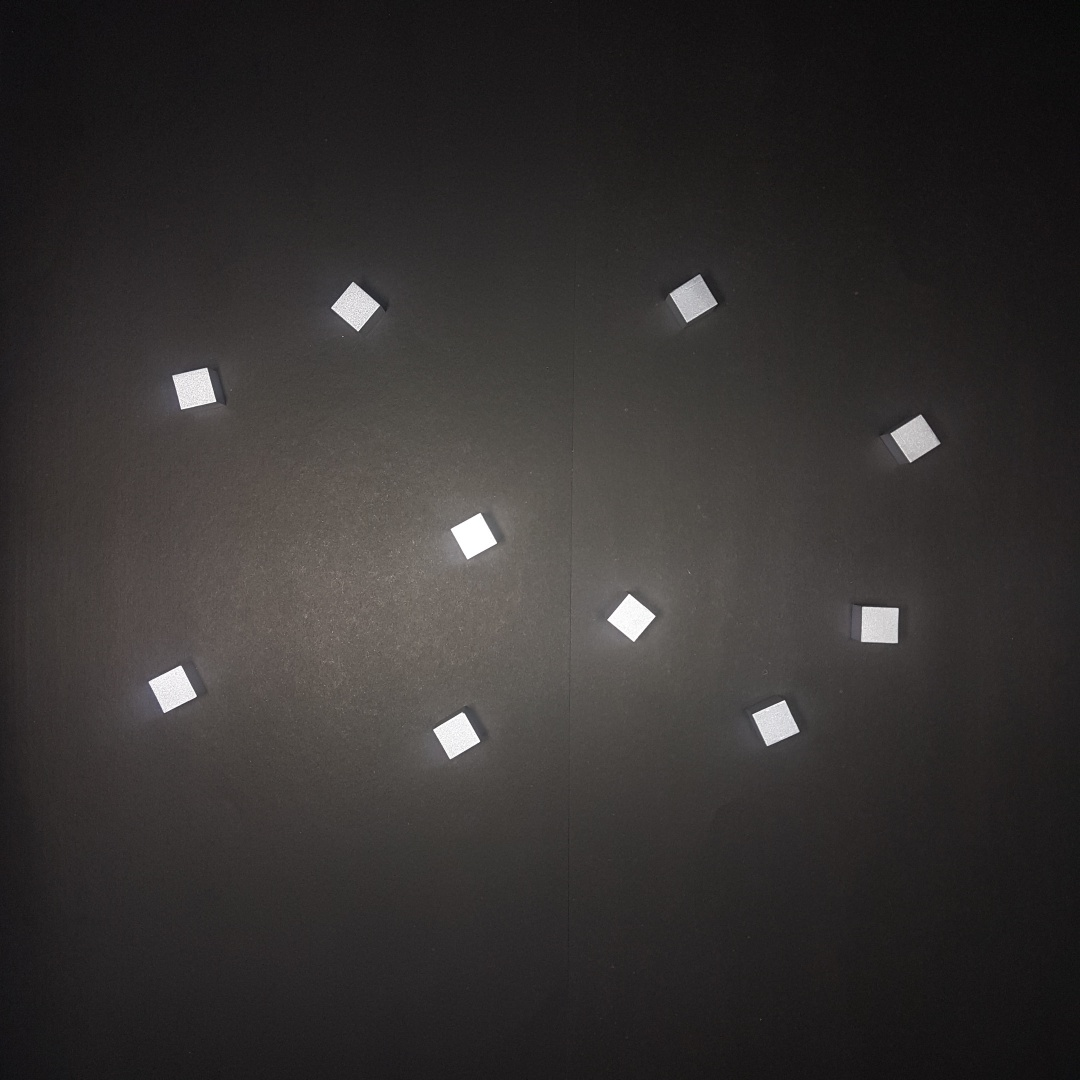
\includegraphics[width=\textwidth]{figures/202106/multiple-cubes.jpg}
         \caption{Top-view of several cubes with bright lighting from above.}
         \label{fig:multiple-cubes}
    \end{subfigure}
    \begin{subfigure}[b]{0.45\textwidth}
         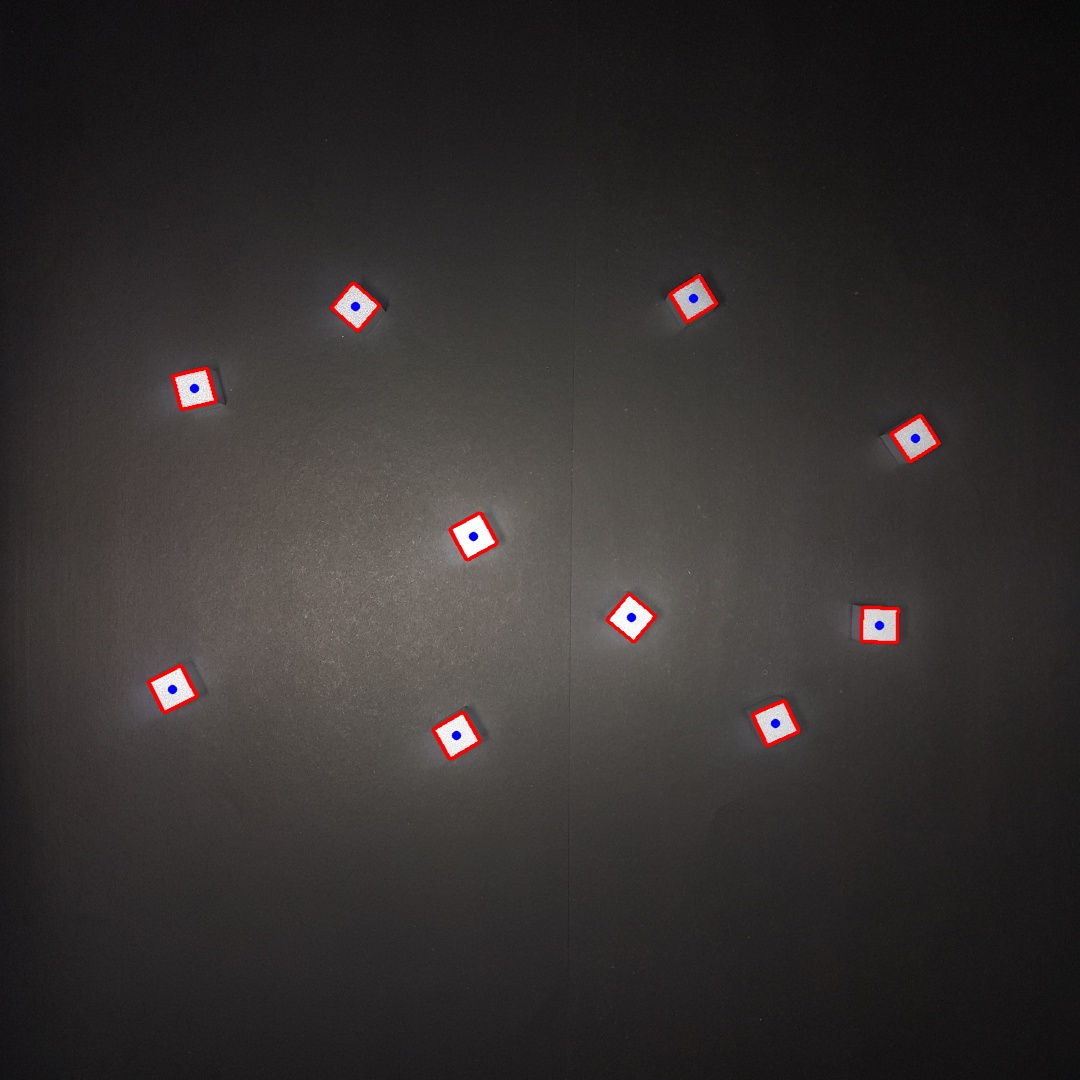
\includegraphics[width=\textwidth]{figures/202106/multiple-cube-centroids.jpg}
         \caption{Output of contour and centroid detection process for cubes in \FigRef{fig:multiple-cubes}.}
         \label{fig:multiple-cube-centroids}
    \end{subfigure}
    \captionsetup{singlelinecheck = false, justification=justified}
    \caption{Centroid detection applied to image containing multiple cubes.}
    \label{fig:multiple-cube-detection}
\end{figure}

\pendsign

\section[2021/06/16]{Thursday, 16 June 2021}

\subsection{Camera Calibration}

The next step in the development of the computer vision subsystem is the mapping of the points in the image coordinate system to coordinates in the world coordinate system. In order to perform this, several parameters about the camera and its orientation need to be known. These parameters can be divided into two categories, namely intrinsic and extrinsic parameters. Intrinsic parameters describe internal properties inherent to the camera itself and include the principal point $(c_x,c_y)$ and the focal lengths ($f_x$ and $f_y$) of the camera. Extrinsic parameters describe the location and orientation of the camera with respect to the world coordinates of the scene and include the rotation and translation transformations that need to be performed to map a point in the world coordinate system to image ecoordinate system. These transformations are captured by the rotation-translation matrix $[\textbf{R}|\textbf{t}]$. Camera calibration is used to estimate the intrinsic characteristics of the camera while camera localisation is used to estimate the extrinsic parameters of the camera \cite{Szeliski2010}. This description is based on the pinhole camera model which is shown in \FigRef{fig:pinhole-camera-model}.

\begin{figure}[!ht]
    \centering
    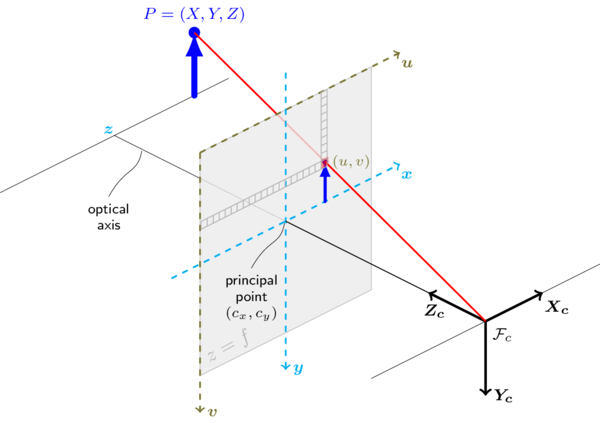
\includegraphics[width=0.7\linewidth]{figures/202106/pinhole-camera-model.png}
    \caption{Diagram showing the parameters of the pinhole camera model. Source: \cite{OpenCVCameraCalibration}}
    \label{fig:pinhole-camera-model}
\end{figure}

The intrinsic parameters of the camera can be expressed as a calibration matrix $\textbf{K}$ as shown in \EquRef{eqn:calibration-matrix} below.

\begin{equation}
    \textbf{K}=
    \begin{bmatrix}
        f_x & s & c_x \\ 
        0 & f_y & c_y \\ 
        0 & 0 & 1
    \end{bmatrix}
  \label{eqn:calibration-matrix}
\end{equation}

The parameter $s$ captures the skew of the sensor axes that occurs as a result of the optical axis not being exactly perpendicular to the sensor plane. However, for practical purposes $s$ can be set to 0. Since the extrinsic parameters are captured by the rotation-translation matrix $[\textbf{R}|\textbf{t}]$, both the intrinsic and extrinsic parameters are captured by the product of this matrix and the calibration matrix $K$. This 3 x 4 product matrix is refered to the camera matrix $P$ and is defined in \EquRef{eqn:camera-matrix} below.

\begin{equation}
    \textbf{P}=\textbf{K}[\textbf{R}|\textbf{t}]
  \label{eqn:camera-matrix}
\end{equation}

The camera matrix is sufficient to map the world coordinates to the coordinates on the image plane provided that the pinhole camera model is used and no lens distortion effects are present. This mapping is captured by \EquRef{eqn:pinhole-camera-mapping} below where $(u,v)$ represent the pixel coordinates on the image plane, $(X,Y,Z)$ represents a point in the world coordinate system and $s$ is simply a scaling factor \cite{OpenCVCameraCalibration}.

\begin{equation}
    s
    \begin{bmatrix}
        u \\ 
        v \\ 
        1
    \end{bmatrix}
    =
    \textbf{P}
    \begin{bmatrix}
        X \\ 
        Y \\ 
        Z \\
        1
    \end{bmatrix}
  \label{eqn:pinhole-camera-mapping}
\end{equation}

Therefore, in order to map the centroids of the cubes from the image coordinate space to the world coordinate space, the intrinsic and extrinsic parameters of the camera need to be determined. Furthermore, real world cameras have lens distortion effects that need to be adjusted for. The OpenCV library was used to perform this camera calibration process to produce the intrinsic parameters of the camera. Furthermore, in order to account for the lens distortion, an improved intrinsic matrix was computed. It must be noted that most literature identifies the camera matrix $P$ as a product of the intrinsic and extrinsic matrices. However, OpenCV refers to the intrinsic matrix $K$ as the camera matrix. 

\begin{figure}[H]
    \centering
    \begin{subfigure}[b]{0.45\textwidth}
         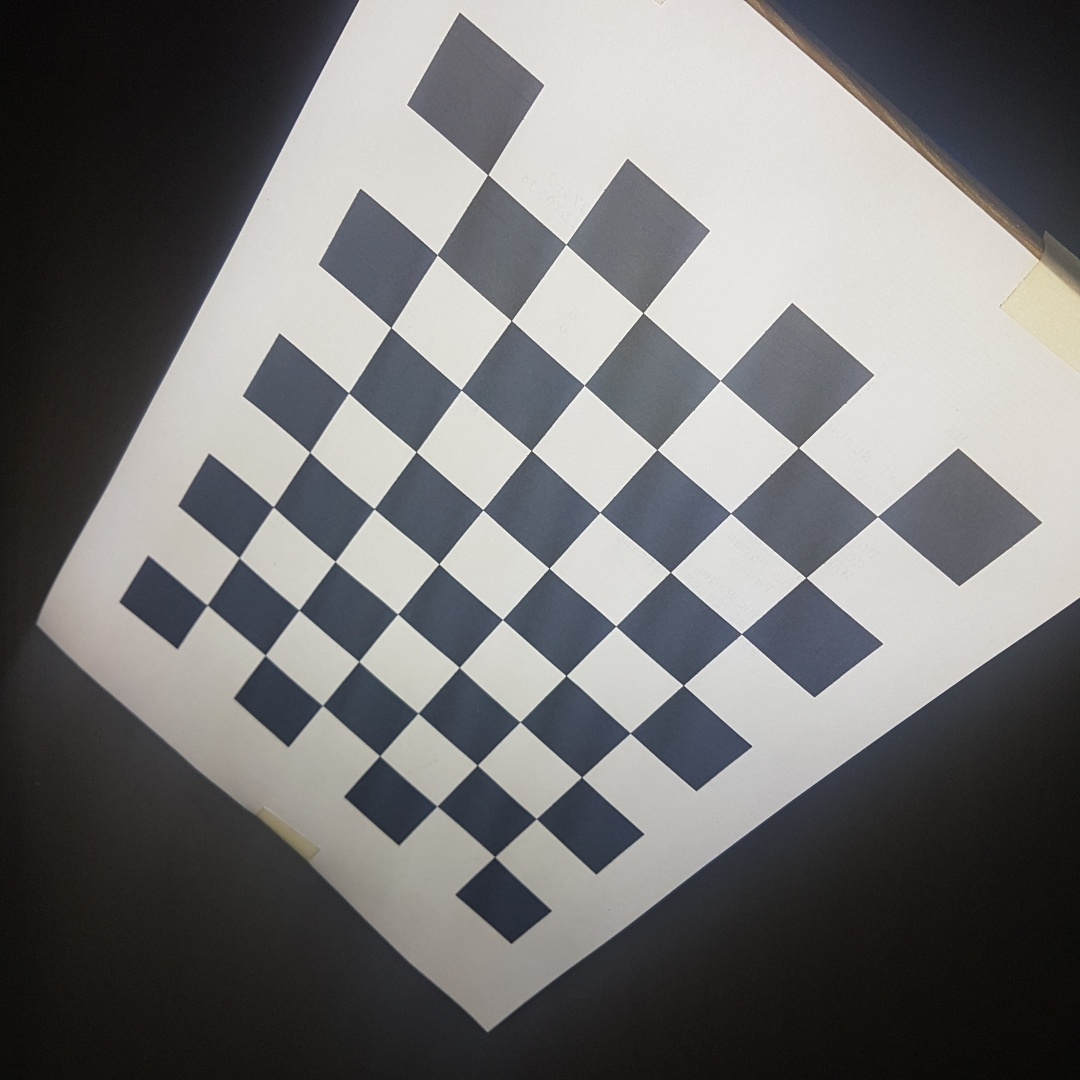
\includegraphics[width=\textwidth]{figures/202106/original-checkerboard.jpg}
         \caption{Checkerboard placed at an angle to facilitate the camera calibration process.}
         \label{fig:original-checkerboard}
    \end{subfigure}
    \begin{subfigure}[b]{0.45\textwidth}
         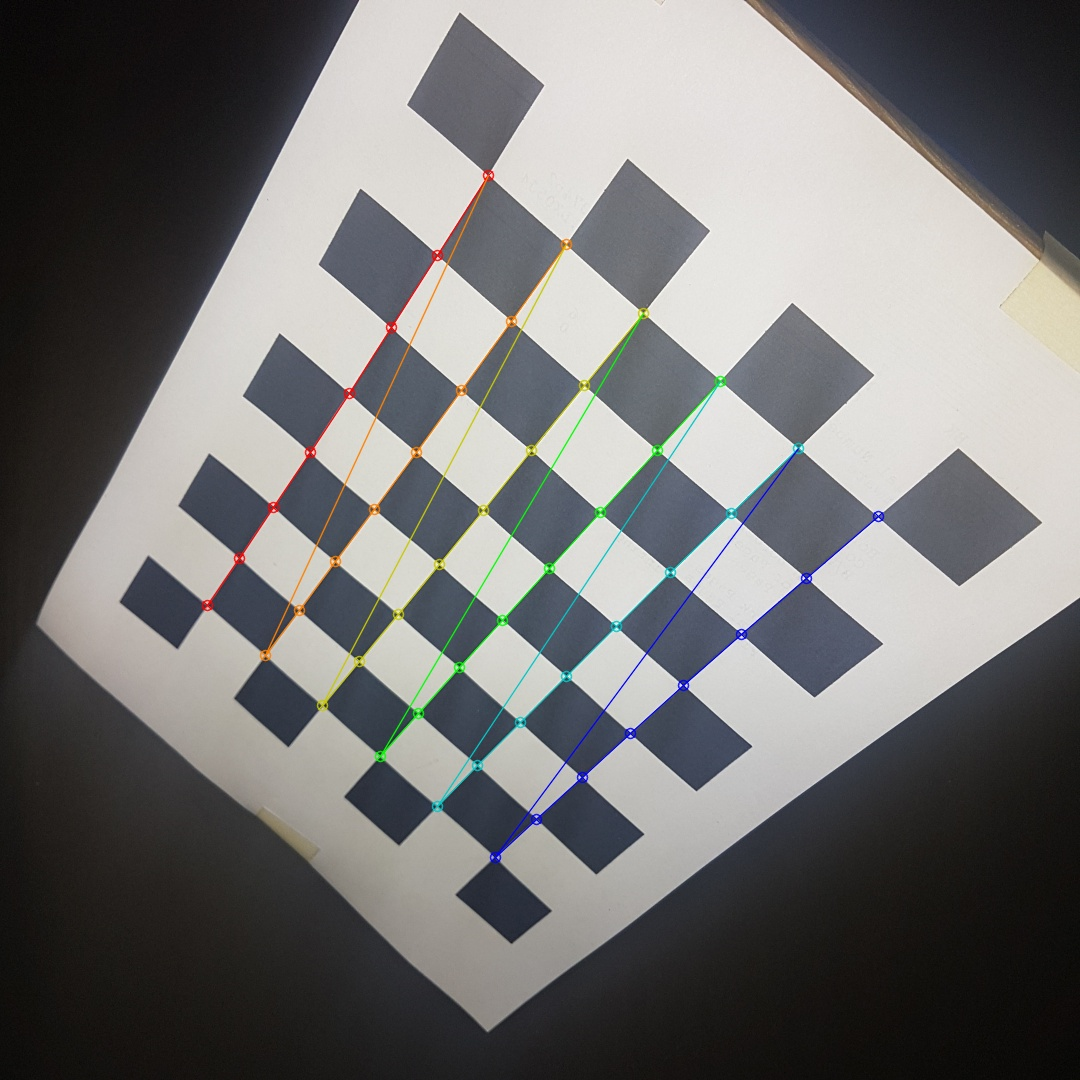
\includegraphics[width=\textwidth]{figures/202106/detected-checkerboard.jpg}
         \caption{\FigRef{fig:original-checkerboard} with various keypoints identified and highlighted.}
         \label{fig:detected-checkerboard}
    \end{subfigure}
    \captionsetup{singlelinecheck = false, justification=justified}
    \caption{Images showing the initial stages of the camera calibration process.}
    \label{fig:checkerboard-calibration}
\end{figure}

In order to perform the camera calibration process and account for the lens distortion, 35 images were taken of a 8x6 checkerboard at various positions and orientations within the camera's \ac{FOV} such as shown in \FigRef{fig:original-checkerboard}. Various known points were subsequently identified on the checkerboard as shown in \FigRef{fig:detected-checkerboard} to facilitate computation of the camera matrix. The improved camera matrix as well as the distortion coefficients describing the tangential and radial lens distortion are used to remap a distorted image as shown in \FigRef{fig:distorted-checkerboard} as to remove the distortion. The undistorted image is shown in \FigRef{fig:undistorted-checkerboard}. Note how the checkerboard lines are perfectly aligned with the red ground truth lines while they are compressed inwards in the distorted image in \FigRef{fig:distorted-checkerboard}.

\begin{figure}[H]
    \centering
    \begin{subfigure}[b]{0.45\textwidth}
        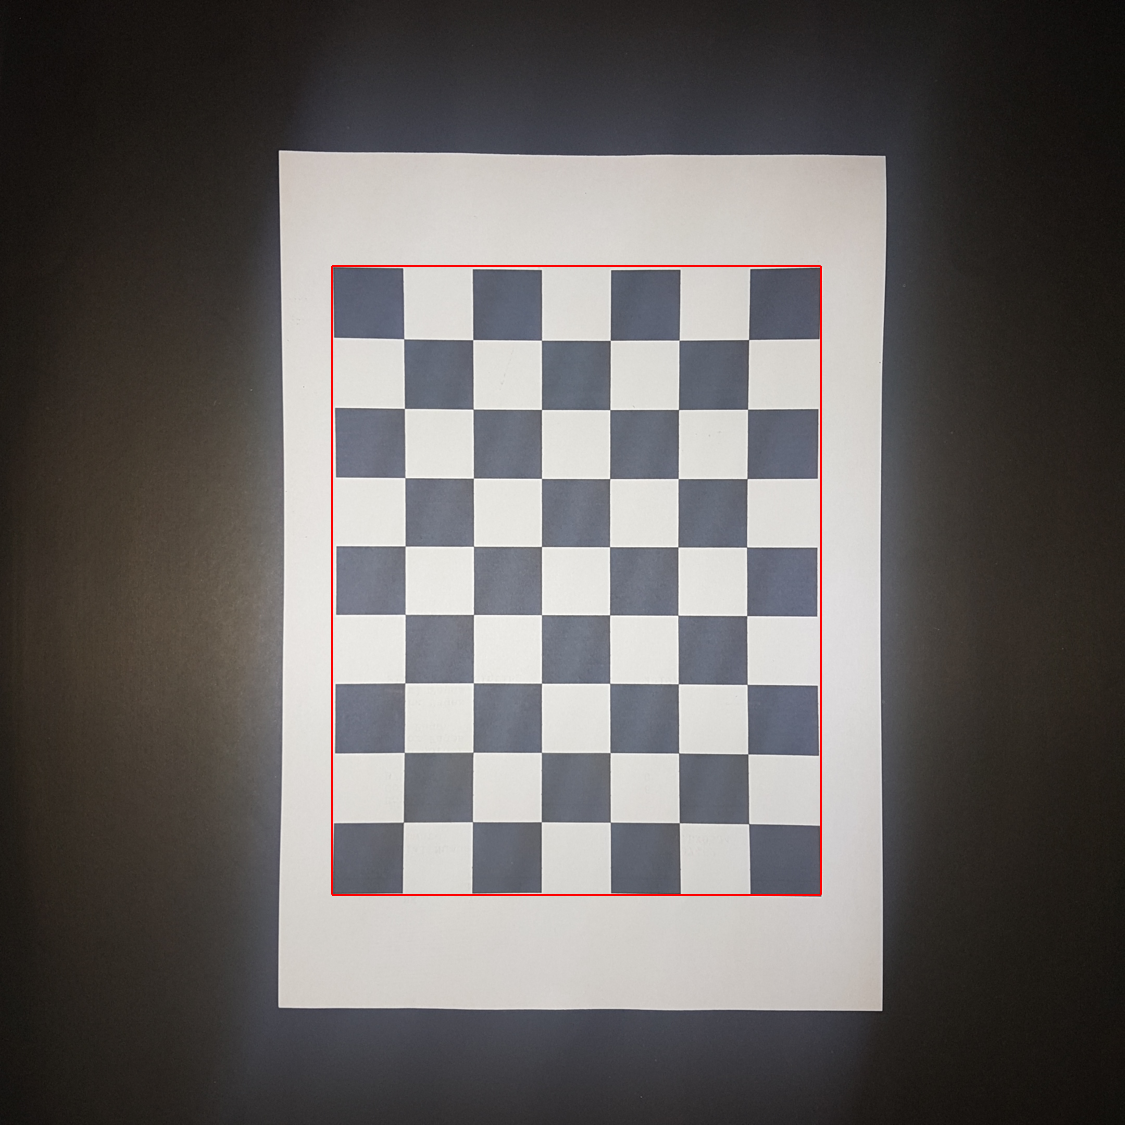
\includegraphics[width=\textwidth]{figures/202106/distorted-checkerboard.png}
        \caption{Original distorted image of the checkerboard.}
        \label{fig:distorted-checkerboard}
    \end{subfigure}
    \begin{subfigure}[b]{0.45\textwidth}
        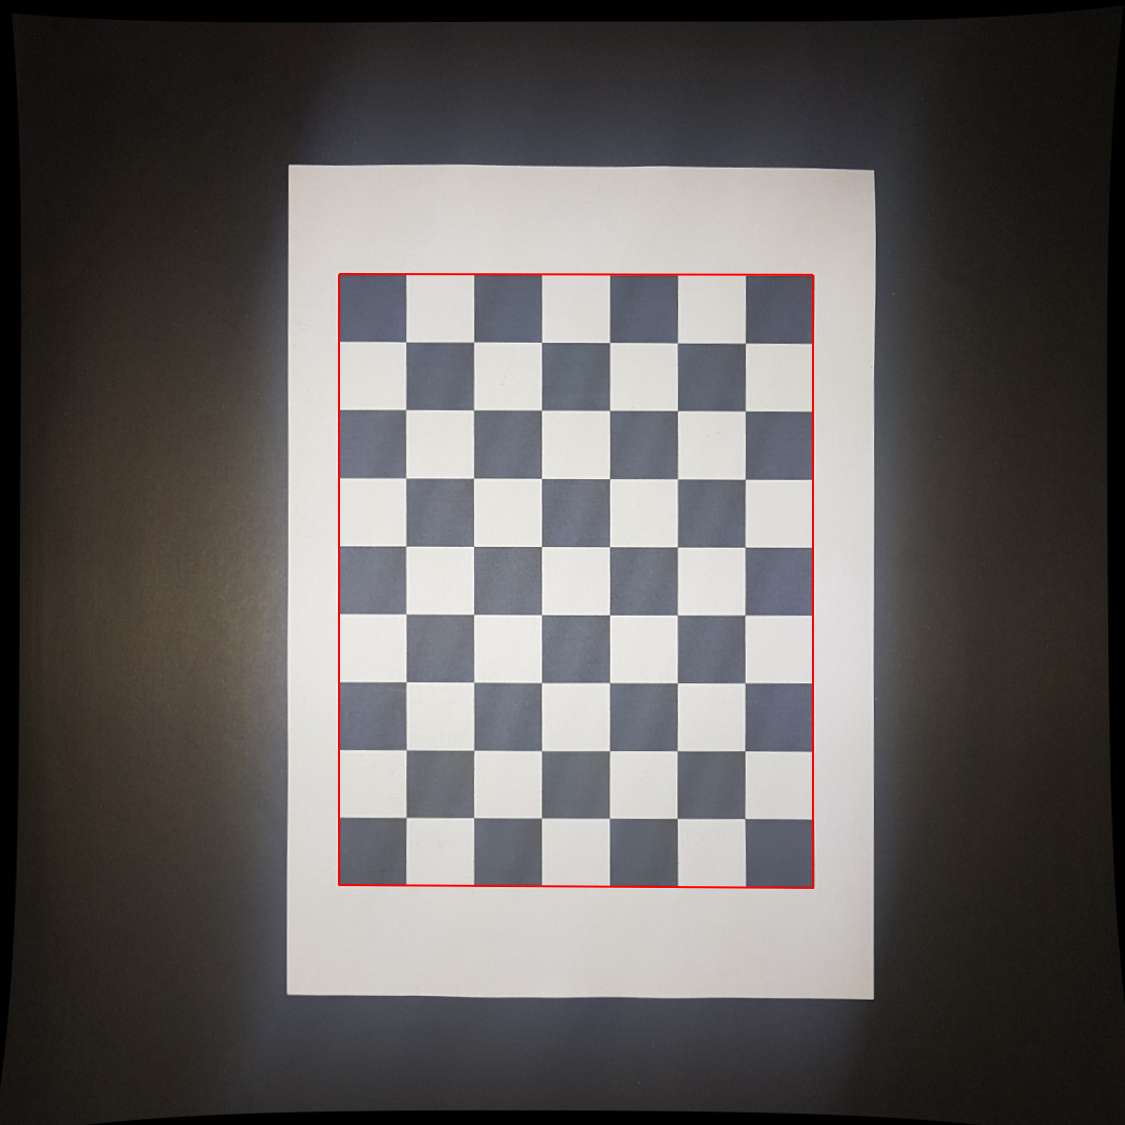
\includegraphics[width=\textwidth]{figures/202106/undistorted-checkerboard.png}
        \caption{Undistorted version of \FigRef{fig:distorted-checkerboard}}
        \label{fig:undistorted-checkerboard}
    \end{subfigure}
    \captionsetup{singlelinecheck = false, justification=justified}
    \caption{Images showing the effect of lens distortion.}
    \label{fig:checkerboard-distortion}
\end{figure}


\pendsign